\section{Test}

\begin{algorithm}[H]
\caption{Lanczos Bidiagonalization}
\begin{algorithmic}[1]
\REQUIRE $A \in \mathcal{R}^{m \times n}$,$k>0$,$\Vert q \Vert_2=1$
\STATE $Q \leftarrow \mathrm{zeros}(n,k+1)$, $Q(:,1) \leftarrow q$
\STATE $P \leftarrow \mathrm{zeros}(m,k)$
\STATE $B \leftarrow \mathrm{zeros}(k,k)$
\FOR{$j=1,2,\cdots,k$}
\STATE $P(:,j) \leftarrow AQ(:,j)$
\IF{$j>1$}
\STATE $P(:,j) \leftarrow P(:,j)-B(j-1,j)P(:,j-1)$
\ENDIF
\STATE Reorthogonalization for $P(:,j)$
\STATE $B(j,j) \leftarrow \Vert P(:,j) \Vert_2$
\STATE $P(:,j) \leftarrow P(:,j)/B(j,j)$
\STATE $Q(:,j+1) \leftarrow A^TP(:,j)-B(j,j)Q(:,j)$
\STATE Reorthogonalization for $Q(:,j+1)$
\STATE $B(j,j+1) \leftarrow \Vert Q(:,j+1) \Vert_2$
\STATE $Q(:,j+1) \leftarrow Q(:,j+1)/B(j,j+1)$
\ENDFOR
\end{algorithmic}
\end{algorithm}

\begin{equation}
  \nonumber
  \begin{array}{C{2cm}|C{4cm}|C{4cm}|C{4cm}}
    \hline
    &\multicolumn{3}{c}{\mathrm{SingularValue\_err}}\\
    \hline
    n&\text{svds}&\text{思路一}&\text{思路二}\\
    \hline
    1000&--&3.3055e-13&1.3848e-13\\
    2000&--&4.7206e-13&2.7108e-13\\
    4000&--&1.7984e-12&3.3993e-13\\
    8000&--&1.4707e-12&8.9585e-13\\
    \hline
  \end{array}
\end{equation}

\begin{figure}[htbp]
\centering
\subfloat[No reconstruction and LF flux]
{
  \label{}% 为子图加交叉引用
  \begin{minipage}{6.5cm}
  \centering
  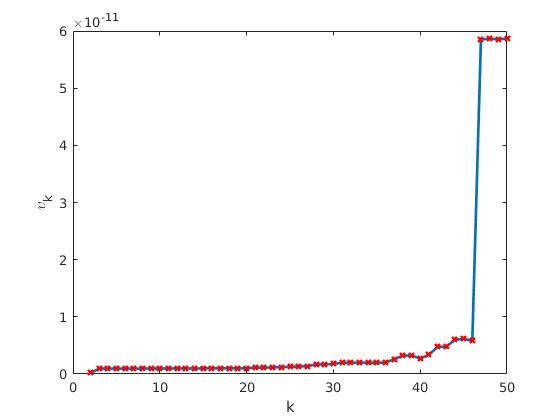
\includegraphics[width=6.5cm]{./pic/1.jpg}
  \end{minipage}
}
\quad
\subfloat[No reconstruction and HLLC flux]
{
  \label{fig:6}
  \begin{minipage}{6.5cm}
  \centering
  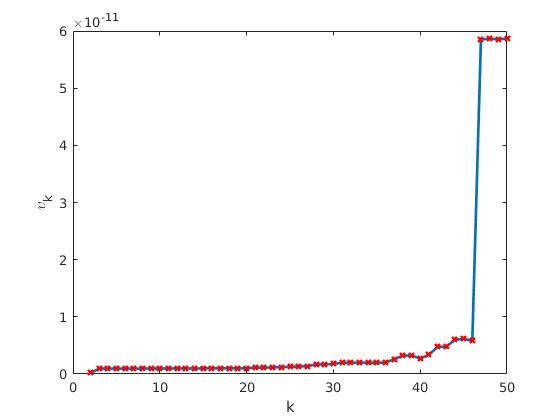
\includegraphics[width=6.5cm]{./pic/1.jpg}
  \end{minipage}
}
\caption{2D Case Results}
\label{fig:9}
\end{figure}